\documentclass{beamer}
\usepackage{beamerthemesplit} % new 
\begin{document}
\title{Control systems} 
\author{Problem-14,IN,GATE-2018} 
\date{\ GUGULOTHU YASHWANTH NAIK(EE18BTECH11017)} 

\frame{\titlepage} 

\section{Problem }
\frame{\frametitle{Problem} 
Consider the transfer function $G(s)=\frac{2}{(s+1)(s+2)}$ . The Phase Margin of $G(s)$ in degrees is
\underline{\hspace{1.5cm}}}

%\frame{\titlepage} 
\section{Solution}
\frame{\frametitle{Solution}
\textbf{Gain Margin:}The gain margin refers to the amount of gain, which can be increased or decreased without making the system unstable. It is usually expressed as a magnitude in dB.
\bigskip
\\Gain Margin = $\frac{1}{|G(j\omega)|}$  at \omega=\omega_{pc}
\bigskip
\\ $\omega_{pc}=$phase crossover frequency (The frequency at which at which phase becomes -180^$^{\circ}$
\bigskip
\\ \textbf{Phase Margin:} Phase margin refers to the amount of phase, which can be increased or decreased without making the system unstable. It is usually expressed as a phase in degrees.
\bigskip


\bigskip

}
\subsection{1 }
\frame{ 
\\ Phase margin =$\phi-\angle(G(j\omega)|_{\omega=\omega_{pc}}$ =$180$^{\circ}$+\phi$
\\ Where , $\phi = \angle G(j\omega)_{\omega=\omega_{gc}}$
\bigskip
\\ $\omega_{gc}=$ The Gain crossover frequency (frequency where Gain becomes 0)
\\Given,  $G(s)=\frac{2}{(s+1)(s+2)}$ 
\bigskip
\\ $\implies$ $ G(j\omega)=\frac{2}{(j\omega+1)(j\omega+2)} $
\bigskip
\\ $\implies$ $ |G(j\omega)|=\frac{2}{(\sqrt{\omega^2+1})(\sqrt{\omega^2+4})} $
\bigskip
\\ $\implies$  $\angle G(j\omega)=-tan^{-1}(\omega)-tan^{-1}(\frac{\omega}{2}) $
}

%\section{Solution}
%\frame{\frametitle{Solution}

%}
\subsection{2}
\frame{ 
\\To find find gain margin we need find $\angle G(j\omega)$

\bigskip 
\\$\angle(G(j\omega)|_{\omega=\omega_{pc}}=-180$^{\circ}$$=$-tan^{-1}(\omega)-tan^{-1}(\frac{\omega}{2})$
\bigskip
\\ $\implies$ $\omega_{pc}=\infty$ $\implies$ Gain margin = $\infty$
\bigskip
\\
\\We have to find phase margin, which is calculated over the gain cross over frequency ($\omega_{gc}$)
\\To find $\omega_{gc}$,
\\We know , Gain=0 at $\omega=\omega_{gc}$
\bigskip
\\$\implies$ $log_{10}|G(j\omega)|=0$ at $\omega=\omega_{gc}$
\bigskip
\\ $\implies$ $|G(j\omega_{gc})|=1$


}
\subsection{3}
\frame{ \bigskip

\\ So, $\frac{2}{(\sqrt{\omega^2_{gc}+1})(\sqrt{\omega^2_{gc}+4})} = 1$
\bigskip
\\ $\implies$ $(\omega^2_{gc}+1)(\omega^2_{gc}+4)=4$
\bigskip
\\ $\implies$ $\omega^4_{gc}+5\omega^2_{gc}+4=4$
\bigskip
\\ $\implies$  $\omega^2_{gc}(\omega^2_{gc}+5)=0$
\bigskip
\\$\therefore \omega_{gc}=0,+j\sqrt{5},-j\sqrt{5}$
\bigskip

}
\subsection{4}
\frame{
\\As frequency is a real quantity
\\Hence, $\omega_{gc} \neq$ Imaginary
\\ So, $\omega_{gc}=0$
\bigskip
\\ $\therefore \angle G(j\omega_{gc})=-tan^{-1}(0)-tan^{-1}(0) = 0$
\bigskip
\\$\implies$ $\phi = 0$^{\circ}$$
\\ $\therefore Phase Margin = 180$^{\circ}$+0$^{\circ}$ $
\bigskip
\\ $\therefore \textbf{Phase Margin = 180$^{\circ}$}$  

}


\subsection{5}
\frame{we can verify the phase margin by bode plot
\begin{figure}
     \centering
      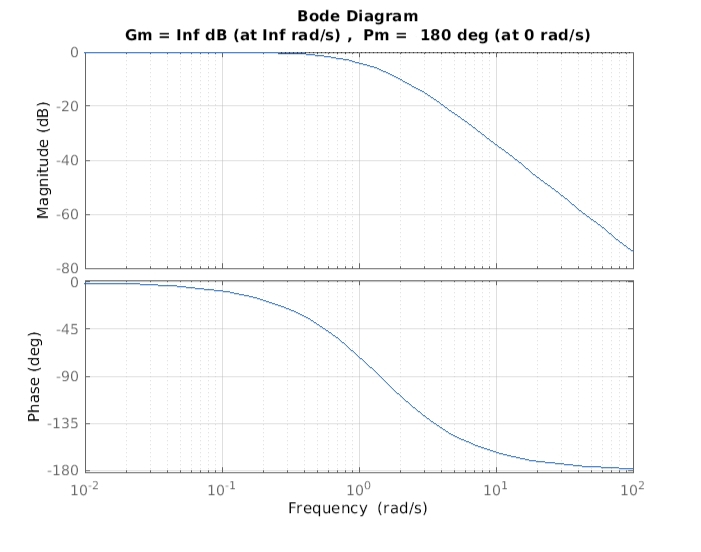
\includegraphics[scale=0.39]{bode.jpg}
\end{figure}
}



}
\end{document}
